\chapter{Architektur}

\section{Systemarchitektur}
neverpile eurekas Systemarchitektur legt den Fokus auf Modularität. Der Kern des Systems beschränkt sich auf die Basis-Funktionalität. Weitere Funktionalität soll in optionalen und austauschbaren Modulen implementiert werden. So konstruierte Softwaremodule werden fortfolgend Facets genannt. Facets in neverpile eureka haben die Möglichkeit strukturell vordefinierte \acs{REST}-Schnittstellen zu implementierten oder auf Lifecycle-Events von Dokumenten zu reagieren.\\
Für die Nutzung gemeinsamer Ressourcen, wie persistentem Speicher oder Indizierungssystemen, werden in Core Interfaces definiert. Diese Anbindungen werden wiederum modular von Facets implementiert und garantieren, dass neverpile eureka ohne harte Abhängigkeiten flexibel in jeder Umgebung eingesetzt werden kann. Die Komposition von Facets, die in einer Instanz von neverpile eureka gemeinsam genutzt werden sollen, können mittels Annotationen und Konfigurationsdateien bestimmt werden.\\
Ein solches Facet ist auch Inhalt dieser Thesis sein. Das Facet, soll für die Auditierung von Dokumenten verantwortlich sein. 

\begin{figure}[!htb]
	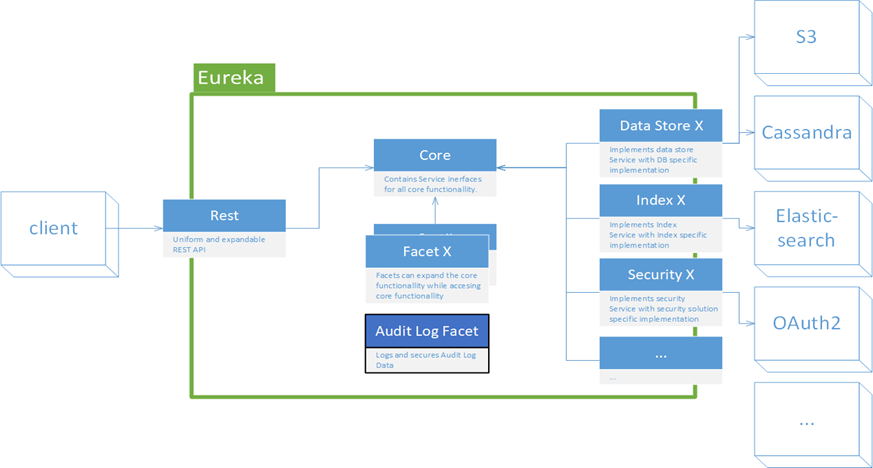
\includegraphics[width=1\textwidth]{content/pictures/eureka}
	\caption{Eureka System Überblick}
	\label{fig:eureka}
\end{figure}

Wie in Abbildung \ref{fig:eureka} dargestellt bietet eureka eine homogene \acs{REST}-Schnittstelle an, welche alle Funktionen zur Verfügung stellt. Eureka nutzt und aggregiert dabei eine Vielzahl bestehender Technologien. 

Das zu implementierende Audit-Facet nutzt dabei alle Möglichkeiten des Eureka Modells. Es werden eigene \acs{REST}-Endpunkte zur Durchführung von Audits angeboten. Das Facet reagiert auf Lifecycle-Events des Dokuments, die das Dokument verändern und nimmt diese Änderungen in das Audit-Log auf. Entsprechende Events sind die Erstellung, die Löschung und die Modifikation von Dokumenten. Über den Core angebotene Ressourcen wie persistenten Speicher und Synchronisationsmechanismen werden ebenfalls zur Erstellung des Audit-Logs verwendet.

\section{Datenmodell}

Für das Audit-Facet werden neue, mit den Dokumenten verknüpfte Daten gespeichert. Die Struktur dieser Daten ist flexibel und kann je nach Anforderung angepasst werden. Fester Bestandteil jeder Implementierung bleibt jedoch das Audit-Event selbst, als kleinste Kerneinheit. Jedes Audit-Log besteht aus vielen dieser Einheiten. Dort sind alle, für das Audit relevanten, Daten über ein einzelnes Ereignis gespeichert. Als eindeutige Identifizierung der Audit-Events wird eine Kombination aus der Dokumenten-ID und einem hochauflösenden Zeitstempel gewählt. Da die Dokumenten-ID einzigartig unter allen Dokumenten ist und jedes Dokument zu jedem Zeitpunkt nur von einem Event verändert werden kann, ist die so generierte ID kollisionsfrei und jedes Audit-Event kann eindeutig identifiziert werden. Auch die ID-Generierung ist modularisiert und kann durch alternative Implementierungen ersetzt werden.\\
Alle Audit-Logs sind fest einem Dokument zugeordnet. So kann ein Audit-Log über ein einzelnes Dokument bezogen werden. Die Beziehung zwischen Audit-Log und Dokument ist lediglich eine Referenz. Die eigentliche Datenstruktur, die alle Audit-Logs zusammenhält, überspannt alle Events.\\
Um Audit-Events zu schützen wird eine Sicherheitsschicht über jedes Audit-Event gelegt. Diese soll garantieren, dass der Inhalt der Events unverändert und konsistent mit allen anderen Events ist. Die genaue Implementierung der Sicherheitsschicht kann mit verschiedenen kryptographischen Strukturen implementiert werden und ist abermals modular und austauschbar.\\
Um eine übermäßig große Anzahl resultierender Audit-Dateien zu vermeiden, werden Audit-Logs in zeitlich abgegrenzte Blöcke aggregiert. Die Referenz von Dokument zu Audit-Event verweist also nicht direkt auf das jeweilige Event, sondern auf den Block, in dem das Event gespeichert ist. Diese Blockstruktur beschleunigt zusätzlich die Verifikation, da so die Anzahl der Speicherzugriffe reduziert wird.

\section{Service Architektur}


\begin{figure}[!htb]
	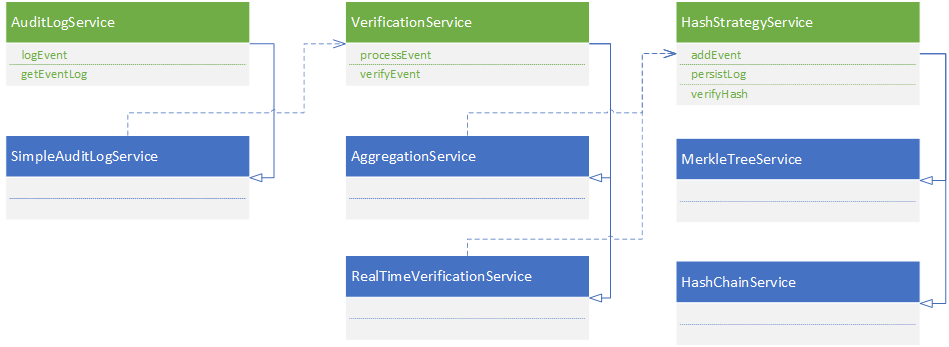
\includegraphics[width=1\textwidth]{content/pictures/services}
	\caption{Service Architektur}
	\label{fig:Services}
\end{figure}

Die Service Architektur des Audit-Log-Facets besteht aus drei Interfaces \label{fig:Services} und deren Implementierungen. 

\subsection{Audit-Log-Service}
Der Audit-Log-Service ist die Schnittstelle zur restlichen Anwendung. Hier werden alle Auslöser für neue Events gesammelt und verarbeitet. Lifecycle-Events werden hier verarbeitet und entsprechende Audit-Events generiert. Die Audit-Events lösen im Allgemeinen das Erstellen eines neuen Eintrags im Audit-Log aus. Auch die \acs{REST}-Ressourcen kommunizieren direkt mit diesem Service. Ein Auditor kann, auf diesem Weg, Verifikationsanfragen für Dokumente, einzelne Events oder das gesamte Log stellen. 

\subsubsection{Implementierung}
Die Lifecycle-Events von Dateien, für die ein Audit-Log erstellt werden soll, können in einer Konfiguration festgelegt werden. Die entsprechenden Events werden anhand dieser Konfiguration gefiltert und verarbeitet. Der Audit-Eintrag wird an den Object Store übergeben, um dieses zu mit Bezug auf den aktuellen Block zu persistieren. Zugleich wird der das Event an den Verification-Service übergeben, um die entsprechende Verifikation zu erstellen. Direkte Anfragen über die Audit-Log-REST-Schnittstelle werden in gleicher Weise an den Objektstore oder den Verification-Service weitergeleitet.

\subsection{Verification-Service}
Der Verification-Service wird vom Audit-Log-Service benutzt und ist sowohl für die Erstellung von Verifikationen als auch für die Verifikation selbst verantwortlich. Des Weiteren wird hier die Verarbeitungsstrategie festgelegt. Die Verarbeitungsstrategie umfasst die Art der Validierung, das Erstellen von Signaturen und die Aggregation von Events. 

\subsubsection{Implementierung}
Für den Verification-Service wurden zwei verschiedene Implementierungen erstellt. Eine erste, simple Implementierung erstellt die Verifikation synchron in der Transaktion, die das Event erzeugt hat. Dieses Verfahren hat neben der Einfachheit den Vorteil, dass die Verifikation innerhalb der Transaktion, die das Event auslöst, erstellt wird. Im Falle eines unerwarteten Fehlers bei der Erstellung der Verifkation, kann so die komplette Transaktion noch unproblematisch abgebrochen oder zurückgerollt werden. Ein weiterer Vorteil ist, dass die Verifikation unmittelbar nach seinem auslösenden Event verfügbar ist.\\
Die alternative Implementierung ist eine Aggregierung von Events zu Blöcken, die dann in einer größeren Transaktion gemeinsam persistiert werden. Vorteil dieser Variante ist die niedrigere Ressourcenanforderung, was einen höheren Datendurchsatz ermöglicht. Da viele Datenhaltungssysteme nicht auf viele kleine Transaktionen optimiert sind, wird diese Variante ab einer bestimmten Last unumgänglich.

\subsection{Hash-Strategy-Service}
Der Hash-Strategy-Service wird vom Verification-Service genutzt. Er bildet ein Interface um die Implementierung der kryptographischen Datenstruktur, deren Erzeugung und Manipulation zu kapseln. Hier werden die Daten für die Sicherheitsschicht, abhängig von der Implementierung, erzeugt und persistiert.

\subsubsection{Implementierung}
Auch für den Hash-Strategy-Service wurden zwei alternative Implementierungen erstellt. Die Erste ist eine Hashchain, die mit einem "`SHA-256"' Algorithmus die Daten der Audit-Events verknüpft. Diese Struktur bietet Flexibilität und ist einfach zu erweitern. Um die Sicherheit der Struktur zu unterstützen und vertrauliche Ankerpunkte in die Kette einzubauen, wird nach konstant vielen Einträgen eine Signatur zum aktuellen Hashwert erstellt. Von diesen Ankerpunkten aus ist die Zugriffszeit maximal $n$, wobei $n$ der Abstand zwischen den Signaturen ist.\\
Die zweite Variante ist eine Kombination aus Merkle tree und Hashchain. Es werden Merkle trees mit fester Größe erstellt. Diese werden wiederum als Hashchain verbunden. Das Verfahren benötigt einen größeren Rechenaufwand zum Erstellen neuer Knoten. Allerdings bietet der Baum Vorteile in Form von Sicherheit durch die höhere Vernetzung der Hashwerte. Die Zugriffszeiten auf ein Log-Event (Blatt) sind binärbaumtypisch logarithmisch. Zudem wird, ähnlich wie bei Hashchains, nach Abschluss jedes Merkle trees eine digitale Signatur der Wurzel erstellt um so alle im Baum enthaltenen Events zusätzlich abzusichern.

\section{Datenfluss}

\begin{figure}[!hbt]
	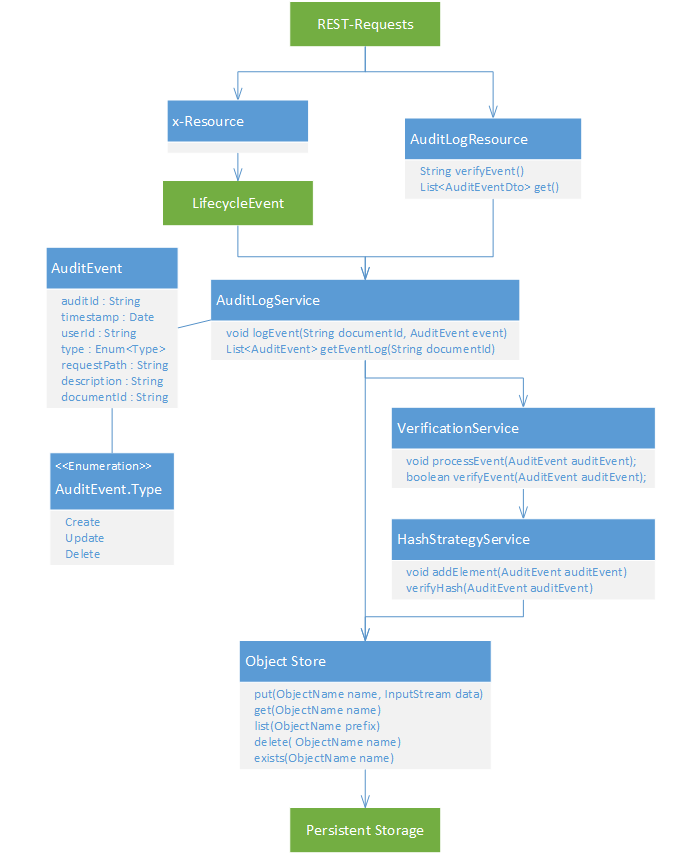
\includegraphics[width=1\textwidth]{content/pictures/auditflow}
	\caption{Anfragen-Fluss}
	\label{fig:auditflow}
\end{figure}

Der Datenfluss des Audit-Log-Facets ist in Abbildung \ref{fig:auditflow} dargestellt. Ausgehend von einer REST-Anfrage kann entweder direkt eine Ressource des Facets angesprochen werden oder eine andere Ressource löst ein relevantes Lifecycle-Event aus. Von diesem Punkt aus wird das Event, wie in der vorigen Sektion beschrieben, von den Audit-Services verarbeitet. Von den Services wird der Object Store genutzt um das Audit-Log selbst und die Verifikation zu persistieren oder bereits abgelegte Daten zu laden.

\section{Cluster-Scaling und Kommunikation}

\begin{figure}[!htb]
	\includegraphics[width=1\textwidth]{content/pictures/instances}
	\caption{Cluster Anfragen-Fluss}
	\label{fig:Instances}
\end{figure}

neverpile eureka ist darauf ausgelegt in einer Container-Umgebung ausgeführt zu werden. Alle Instanzen eines neverpile eureka Cluster sind gleichwertig. Die Instanzen haben alle einen identischen Umfang und Zuständigkeitsbereich. Es gibt keine Hierarchie und auch keine Abhängigkeiten zwischen Instanzen. Durch diese Homogenität ist ein On-Demand Scaling ein einfaches Zuschalten beliebig vieler weiterer Instanzen. Jede Anfrage an die \acs{API} wird von einem Loadbalancer entgegengenommen und dann an eine beliebige Instanz weitergeleitet (siehe Abbildung \ref{fig:Instances}). Die Kommunikation zwischen Instanzen ist minimal, wodurch diese unabhängig voneinander Anfragen bearbeiten können. Dieses Clustersystem erlaubt einfache Skalierung bei steigenden Anforderungen.

\section{Distributed processing}
Auch wenn die Instanzen von neverpile eureka so unabhängig voneinander arbeiten sollen wie es möglich ist, kommt man beim Thema Audit-logging nicht gänzlich um eine Synchronisation zwischen den Instanzen aus. Bei der Verifikation ist die Reihenfolge essenziell. Wenn mehrere Instanzen gleichzeitig Audit-Events auslösen, muss daher sichergestellt werden, in welcher globalen Reihenfolge die Events geordnet werden. Sich nur auf Timestamps zu verlassen ist in diesem Fall nicht ausreichend, da es zu identischen Timestamps kommen kann und die Synchronisation der lokalen Uhren der Instanzen nicht garantiert werden kann. Wenn also die rein zeitliche Bestimmung der Reihenfolge nicht zielführend ist, müssen komplexere Methoden verwendet werden. Die gewählte Lösung ist ein leichtgewichtiges Protokoll zwischen den Instanzen. Das Protokoll wird bereits an anderen Stellen in neverpile eureka verwendet und erzeugt deshalb keine zusätzlichen Abhängigkeiten. 
"`Distributed in Memory computing"' wird von vielen renommierten Frameworks benutzt und erlaubt es Daten zwischen Instanzen zu synchronisieren und atomare Operationen auf diesen auszuführen. Für die Implementierung der Lösung kann auf einige erprobte Open-Source-Lösungen, wie Apache Ignite oder Hazlecast, zurückgegriffen werden. Passend zum Gesamtkonzept von neverpile eureka werden keine Technologien vorgegeben. Es werden stattdessen Interfaces entwickelt, die mit einer frei gewählten Technologien implementiert werden können. Die einzige Anforderung des Audit-Logs, die Kommunikation zwischen den Instanzen erfordert, ist das Lösen des Total-Ordering-Problems. Dazu wird eine Distributed Atomic Reference verwendet. Diese Referenz wird zwischen allen Instanzen repliziert und der Zugriff reguliert. In dieser Referenz wird das neueste Event gespeichert. Die synchronisierte Referenz kann mit einer atomaren Funktion von jeder Instanz mit einem neuen Event aktualisiert werden. Durch die Referenz ist gewährleistet, dass alle Instanzen mit dem aktuellen Hash arbeiten und sich unmissverständlich auf eine Reihenfolge einigen.\cite{7496608}
